\documentclass{beamer}
\mode<presentation>{\usetheme{AV}}
\usepackage{etex}
\usepackage[export]{adjustbox}
\usepackage{epsfig}
\usepackage{feynmp}
\usepackage{verbatim}
\usepackage{listings}
\usepackage{colortbl}

\usepackage{color}

\definecolor{mygreen}{rgb}{0,0.6,0}
\definecolor{mygray}{rgb}{0.5,0.5,0.5}
\definecolor{mymauve}{rgb}{0.58,0,0.82}

\usepackage[utf8]{inputenc}
\usepackage[T1]{fontenc}
\usepackage{lmodern}
\usepackage{amsfonts}
\usepackage{supertabular}

\usepackage{textcomp}
\usepackage{amsmath}
\usepackage{amssymb}
\usepackage{graphicx}
%\usepackage{wrapfig}
\usepackage{subfigure}
\usepackage{type1cm}
\usepackage{tikz}
\usepackage{tikz-3dplot}
\usepackage{tikz}
\usepackage{tikz-3dplot}
\usepackage{pgfplots}
\usepackage{ulem}
\usetikzlibrary{shapes,arrows}
\usepackage{pgfplots}
\usetikzlibrary{shapes,arrows}
\usepackage{rotating}%     - to rotate boxes, pictures etc.
\usepackage{amsmath}%      - to use the AMS extended math package
\usepackage{amssymb}%      - to obtain additional math symbols in AMS fonts
\usepackage{amscd}%        - to obtain AMS flow chart utilities
\usepackage{array}%        - to obtain additional tabular functionality
\usepackage{multirow}%     - for multirow-entries in tables
\usepackage{supertabular}% - for multi-page tables
\usepackage{dcolumn}%      - decimal-point aligned colums in tables
\usepackage{xspace}%       - to add empty space after commands
\usepackage{upgreek}%      - provide upright greek letters
\usepackage{calc}%         - enhanced calculus in LaTeX macros
\usepackage{ifthen}%       - enhance logical structures in LaTeX macros
\usepackage{cite}%         - for multiple citations like [1-4] instead of [1,2,3,4]
\usepackage{tikz} 
%\usepackage{enumitem} 
\usepackage{multirow}
\usepackage{amssymb}
\usepackage{mathtools}
\usepackage{graphicx}


\def\Tiny{\fontsize{4.0pt}{4.0pt}\selectfont}

\title[DPHEP2017]{2nd DPHEP Collaboration Meeting}
\subtitle[DPHEP2017]{DPHEP2017}
\author[Andrii Verbytskyi]{
Andrii Verbytskyi
}
\date[]{\\ \today}


\setbeamersize{text margin left=.3cm,text margin right=.3cm} 
\listfiles
\begin{document}

\usebackgroundtemplate{%
  \tikz\node [anchor=north east, inner sep=0pt,opacity=0.18]  at (current page.center)
     {\includegraphics[height=0.5\paperheight,width=\paperwidth]{bkg3.eps}};
}

\frame{
\vspace{0.3cm}
\begin{figure}

\includegraphics[height=1.0cm]{eps/MPP_os_logo_cmyk.eps}
%\includegraphics[height=1.0cm]{eps/CERN-Logo-cyan-RGB_ger.eps}
\hspace*{12.0cm}
\end{figure}
\begin{center}
\vspace{1.3cm}
{\LARGE The OPAL long term data preservation project in Max-Planck Institute f\"{u}r Physik and more}
\vspace{0.3cm}
\end{center}
\begin{center}
\vspace{0.3cm}
Andrii Verbytskyi\\
\end{center}
\vspace{1.0cm}
\begin{center}
\footnotesize  2nd DPHEP Collaboration Meeting \\Geneva,\\ \today
\end{center}
\vspace{0.4cm}
}


\usebackgroundtemplate{%
  \tikz\node [anchor=north east, inner sep=0pt,opacity=0.98]  at (current page.center)
     {\includegraphics[height=1.0\paperheight,width=\paperwidth]{LEP2}};
}


\frame{\frametitle{LEP}
{\color{white}\Large\bf 
\begin{itemize} 
\item \color{white}Electron-positron collider, 27km ring, started in CERN (1989-2000); 
\item \color{white}Beam energies 45-105GeV;
\item \color{white}Experiments: ALEPH, DELPHI, L3, {\color{red}OPAL}.
\end{itemize} 
} 
}
\usebackgroundtemplate{}

\frame{\frametitle{OPAL}
\begin{centering}
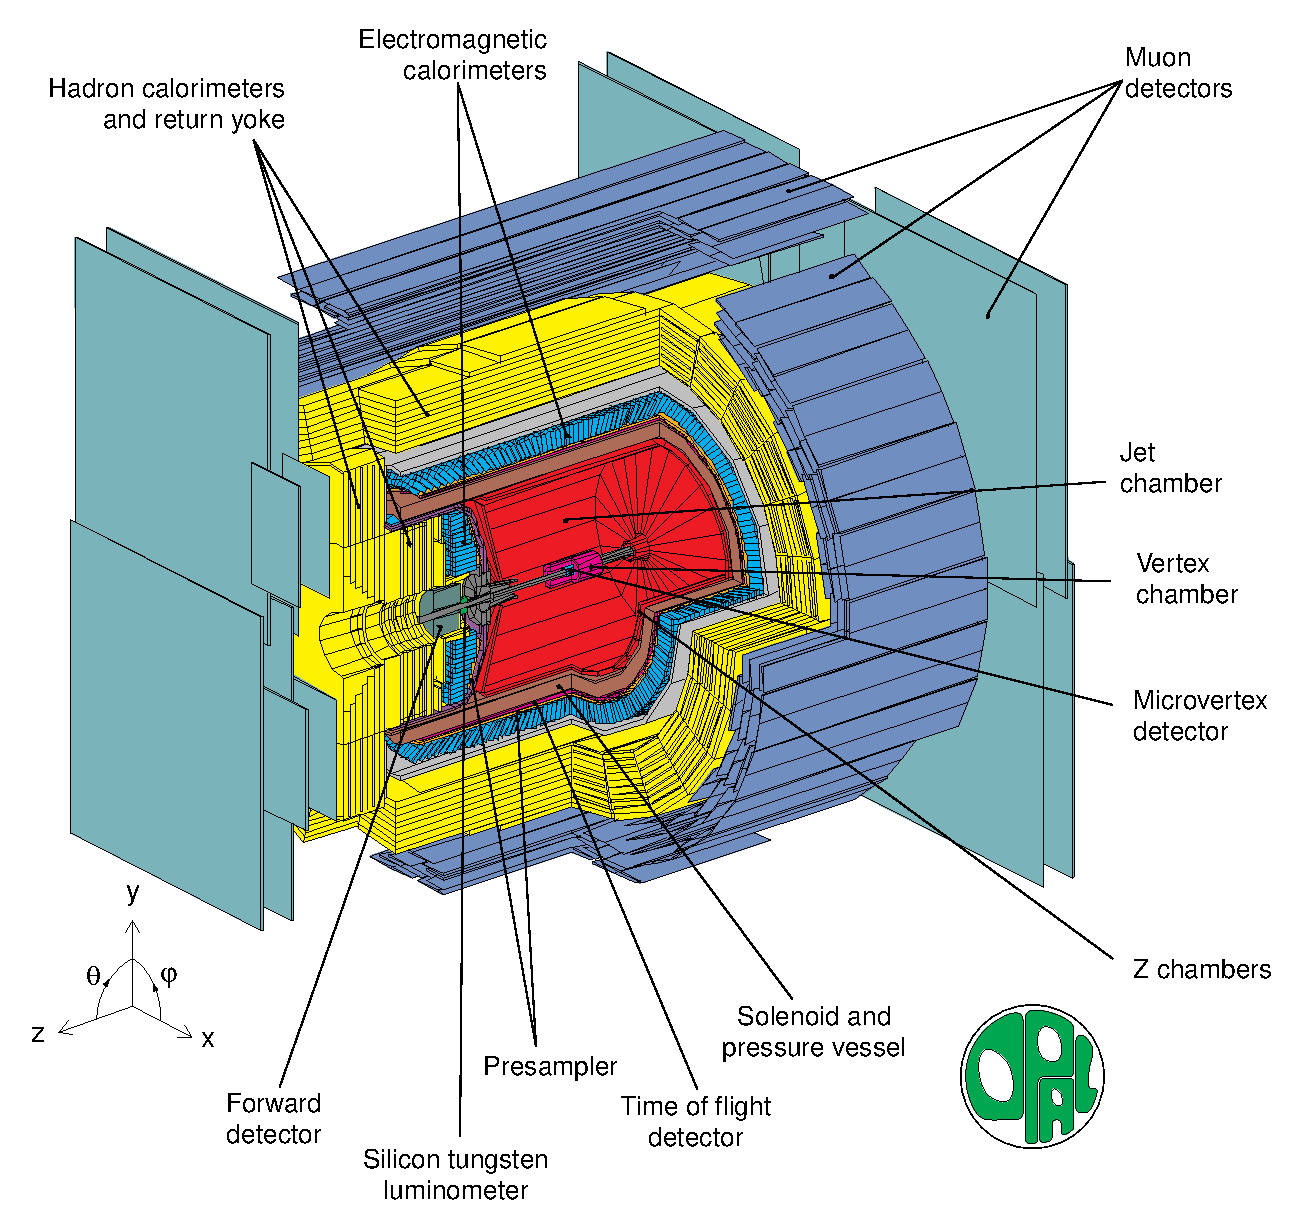
\includegraphics[width=0.8\linewidth]{opal_3d_colour}	
\end{centering}
%\begin{columns}[c]
%\column{0.49\linewidth}
%\begin{itemize} 
%\item multipurpose detector 
%\item large solid angle coverage
%\item digital readout
%\end{itemize} 
%\column{0.49\linewidth}
%\begin{itemize} 
%\item advanced tracking system
%\item calorimeter
%\item muon chambers
%\end{itemize} 
%\end{columns}
%{\bf \color{red} 35 years later: still unique energy range coverage!}
}


%eps/OPALDet.eps

\usebackgroundtemplate{%
  \tikz\node [anchor=north east, inner sep=0pt,opacity=0.18]  at (current page.center)
     {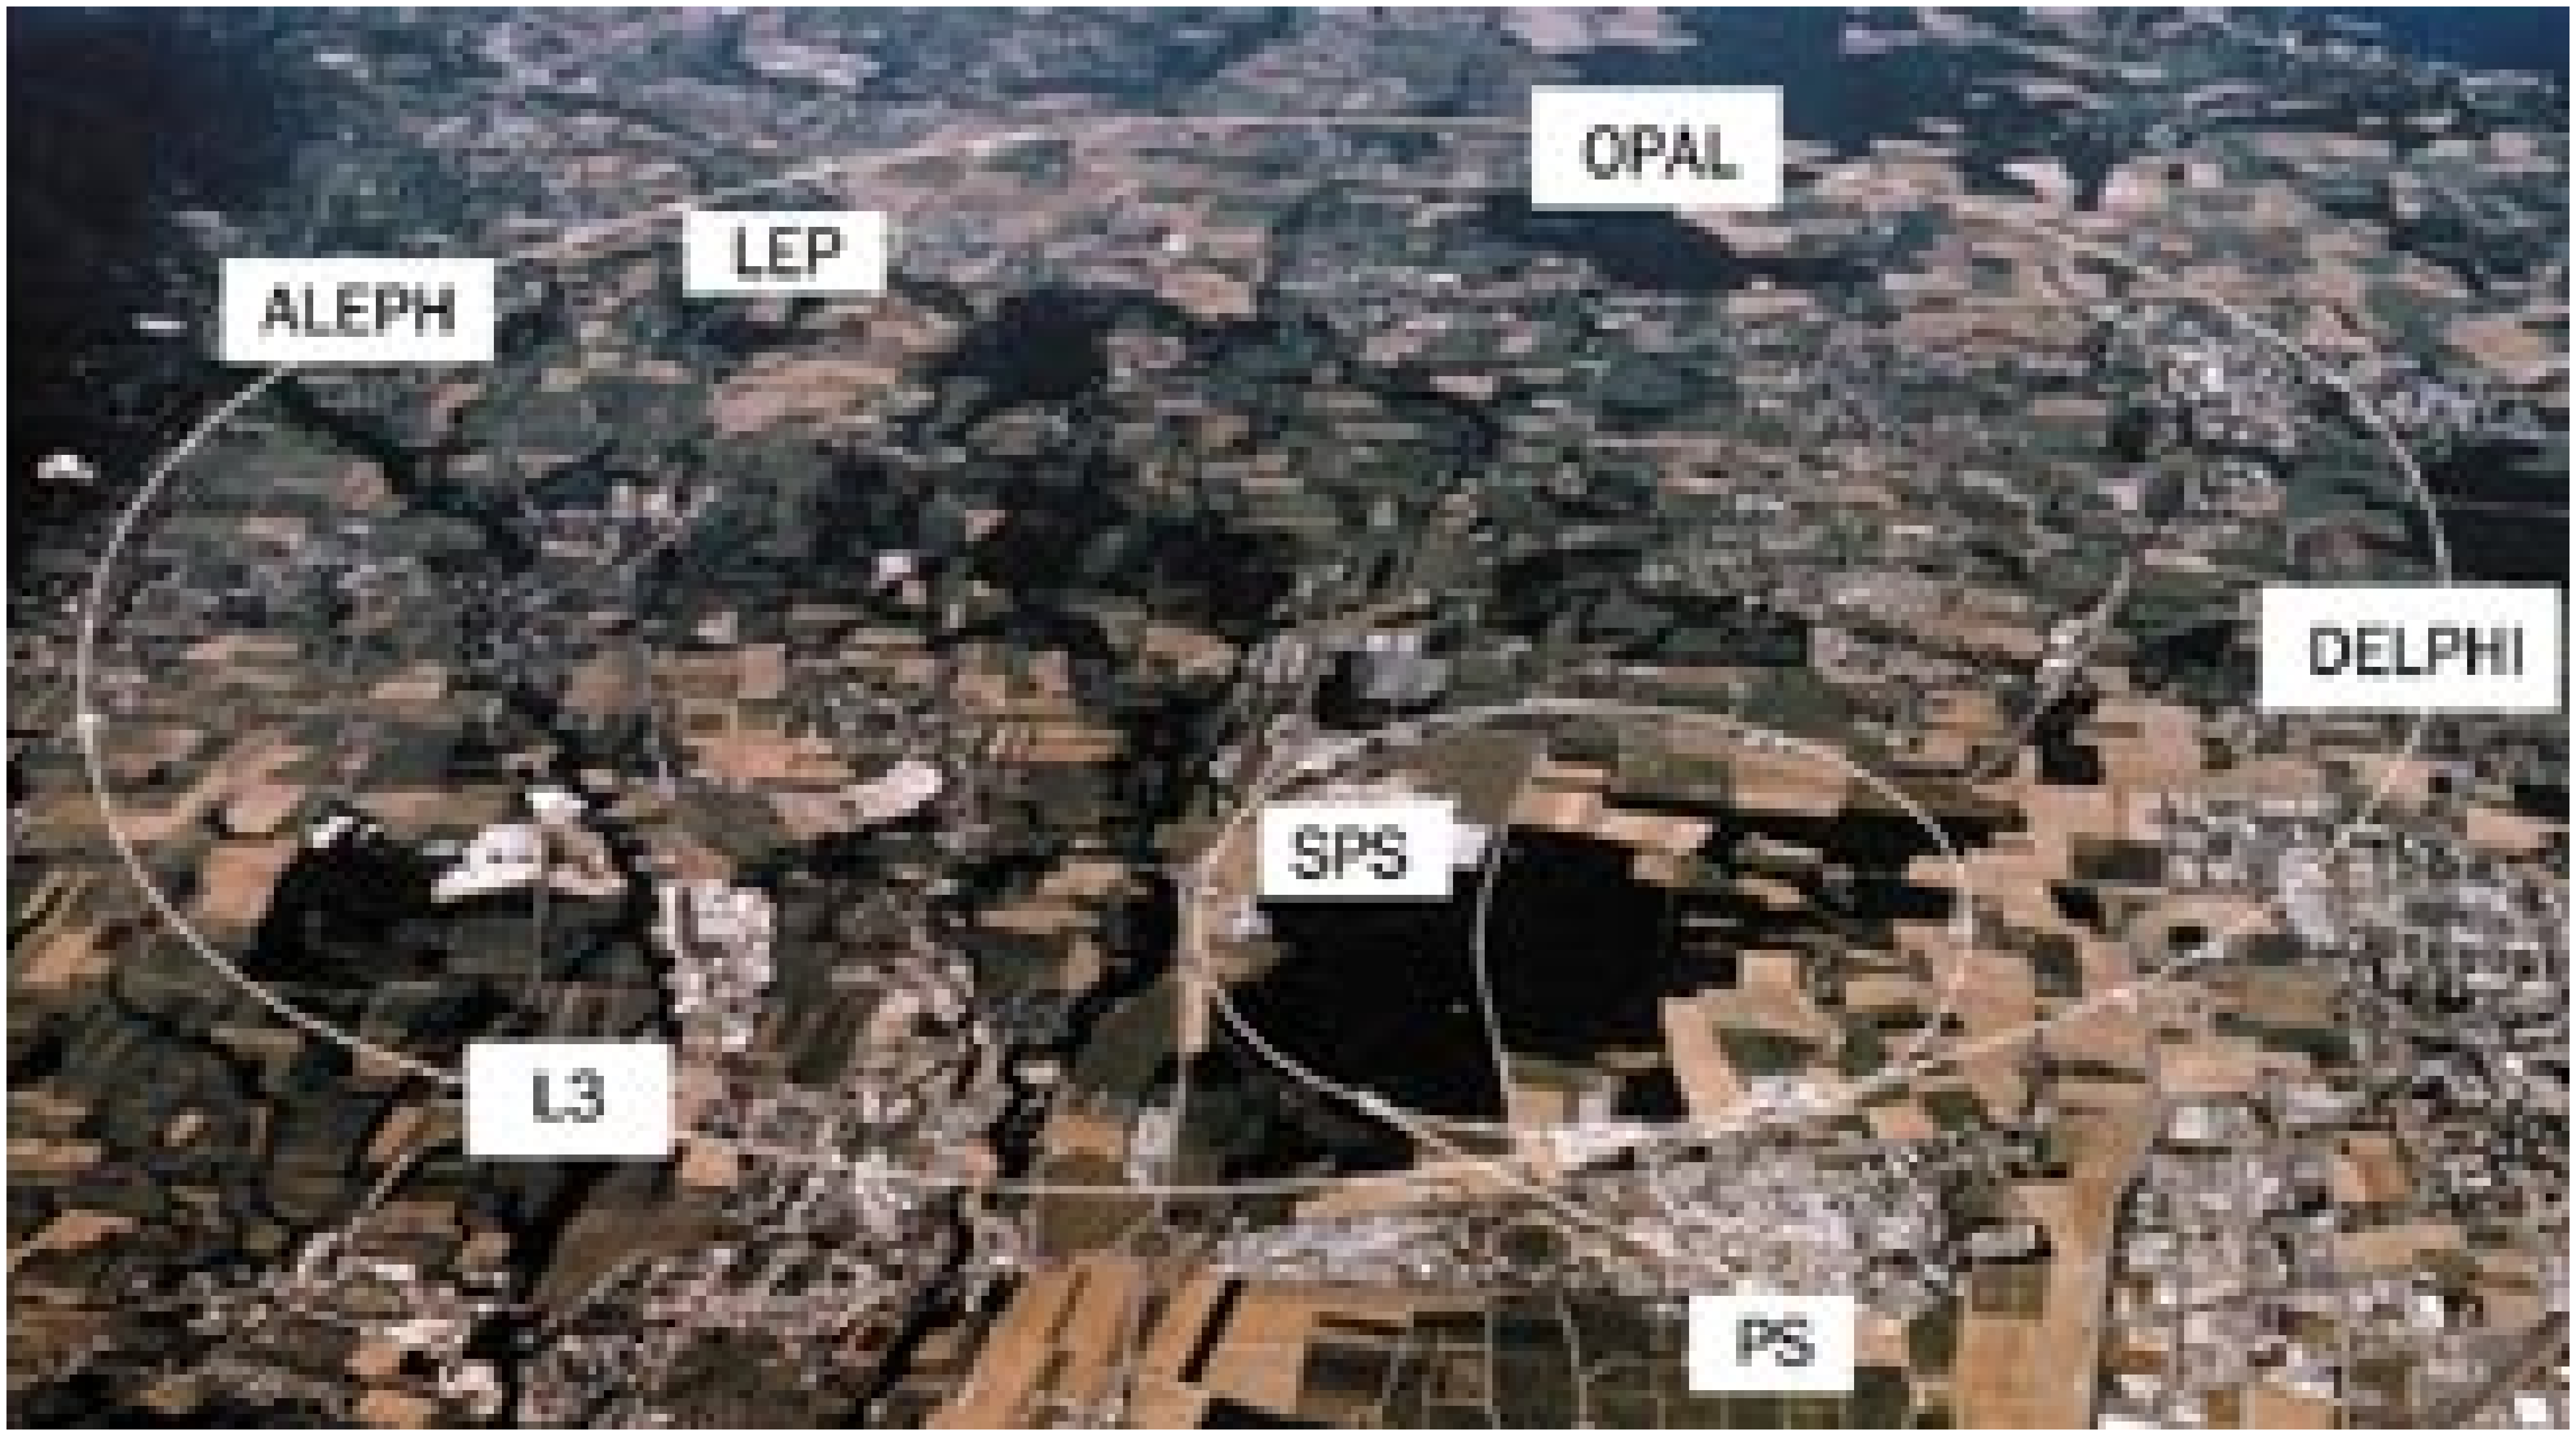
\includegraphics[height=1.0\paperheight,width=\paperwidth]{LEP}};
}


\frame{\frametitle{OPAL  and data preservation}
\begin{columns}[c]
\column{0.54\linewidth}
OPAL@LEP reminder:
\begin{itemize}
\item Precision QCD;
\item Electroweak physics;
\item Flavour physics;
\item Searches (also Higgs)\dots
\end{itemize}
Motivation for data preservation:
\begin{itemize}
\item Future data (re-)analysis with new models and new approaches.
\item Modelling for the future experiments.
\end{itemize}
\column{0.45\linewidth}
\begin{itemize}
\item 5M events.
\item 400k hadronic events at LEP-II (91-210GeV)
\end{itemize}
%\includegraphics[width=1.0\linewidth]{eps/OPAL-ID-records.eps}
\end{columns}
}

\usebackgroundtemplate{}








\frame{\frametitle{MPP DP  model for OPAL}
\begin{columns}[c]
	\column{0.6\linewidth}
{\bf Data preservation is about  new and interested results with old data.}
{\bf In addition  the Data Preservation  experience with OPAL has an extreme importance on itself.}\\
In out model we describe  ingredients and tools:\\
\column{0.4\linewidth}
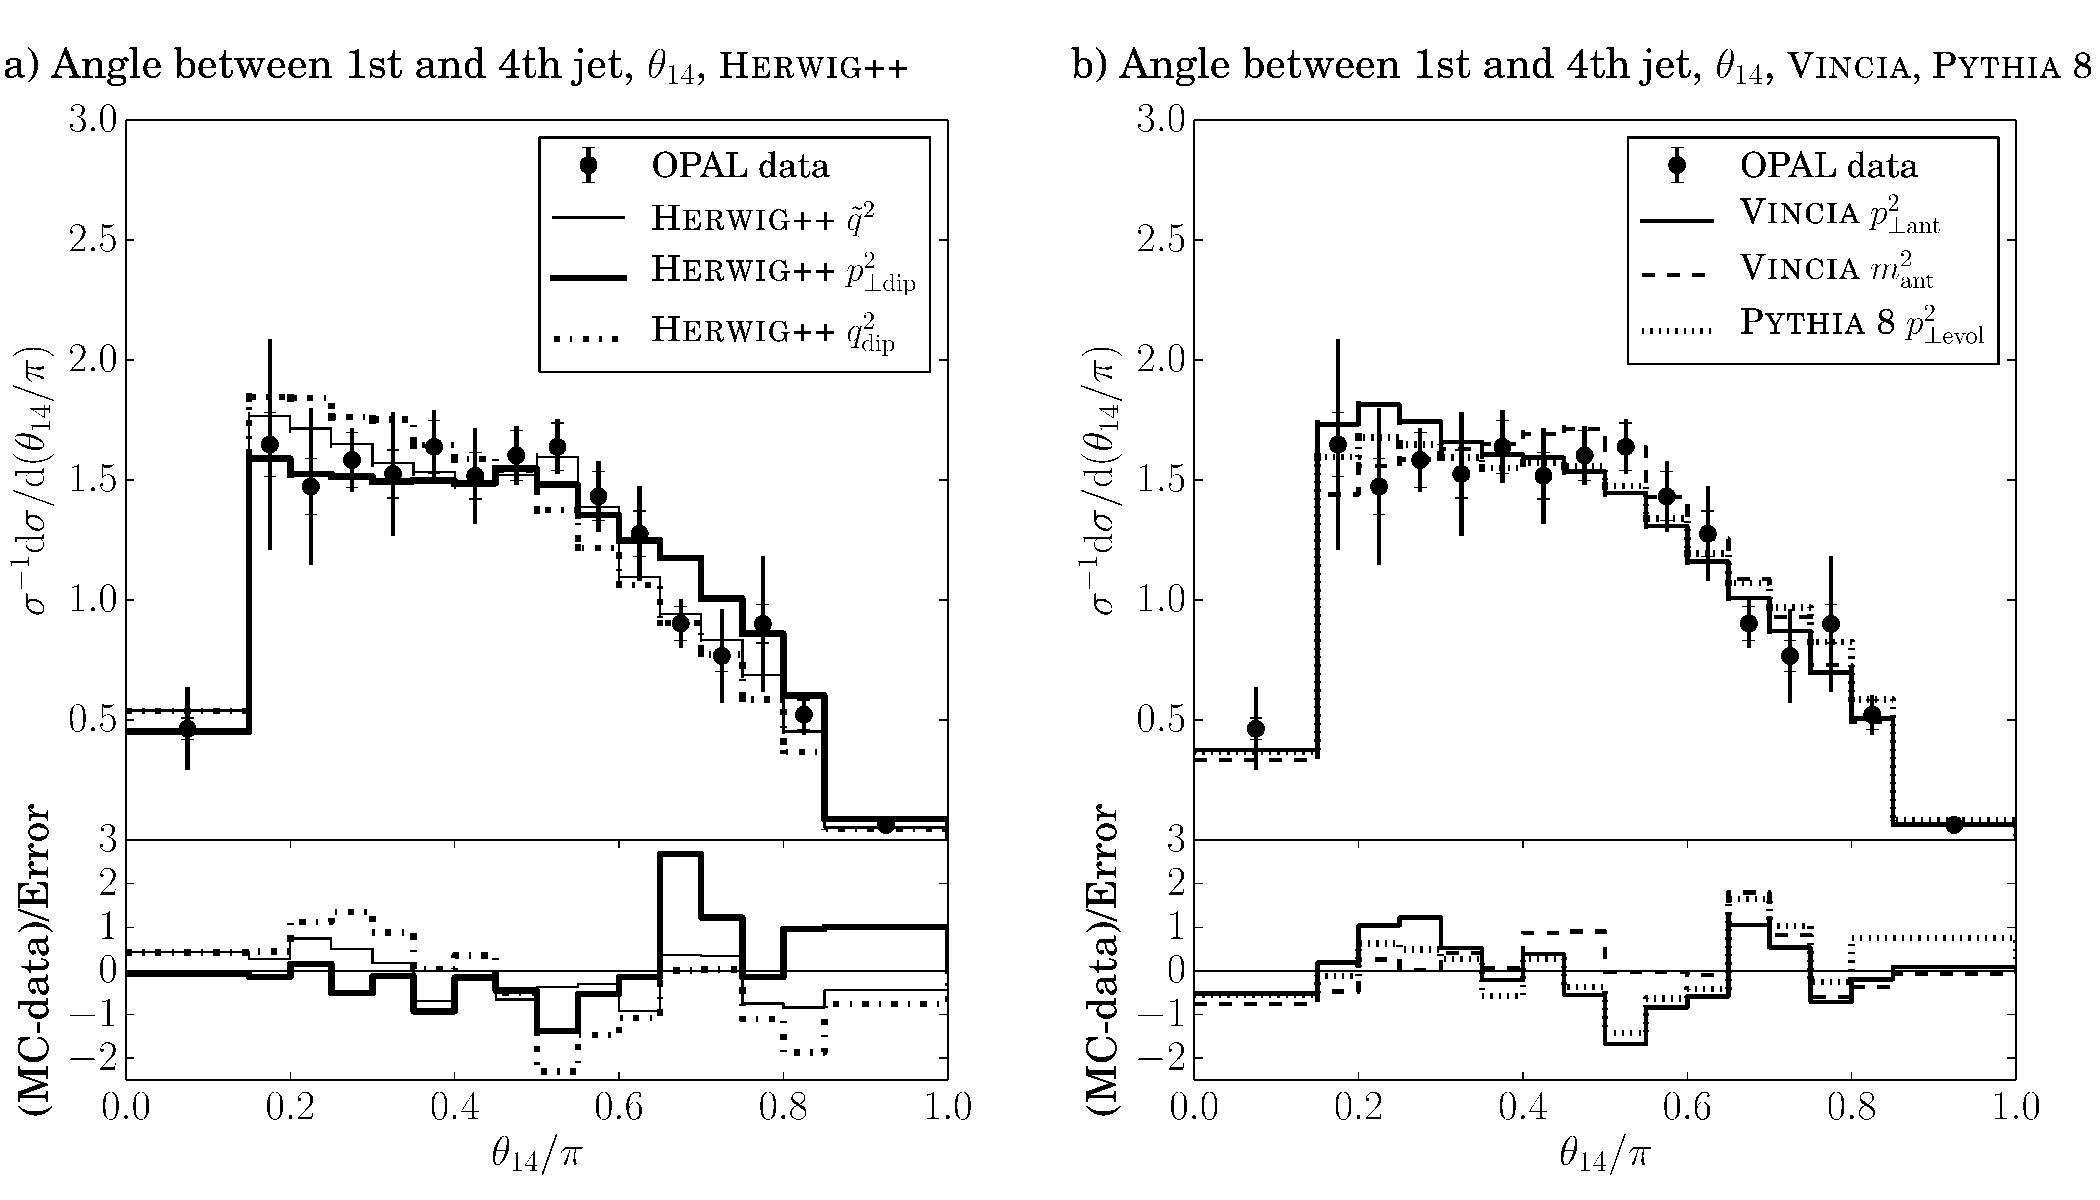
\includegraphics[width=1.0\linewidth,height=0.85\linewidth]{A14.ps}\\
Eur.Phys.J. C75 (2015) no.12, 571
\end{columns}
\begin{columns}[c]
\column{0.4\linewidth}
\begin{itemize}
\item Data bits
\item Software
\end{itemize}
\column{0.6\linewidth}
\begin{itemize}
\item Experiment documentation
\item DP policies and  documentation
\end{itemize}
\end{columns}

\begin{itemize}
\item But in the end we are interested in {\bf physics }.
\end{itemize}

Main idea: enable physics and make it doable with modern methods in modern environments with minimal effort.\\
}



\frame{\frametitle{MPP DP model for documentation  and policies}
%MPP data preservation relies on the documentation preserved as papers by CERN/CERN library/InSpire.\\
\begin{itemize}
\item OPAL publications are available in InSpire, journals, arXiv or in CERN.
\item The non-digital documentation is preserved in CERN.
%\item Logbooks included!
%\item Some available online as well, see details at https://wwwOPAL.mpp.mpg.de/
\end{itemize}
\begin{figure}\centering
%\includegraphics[width=0.3\linewidth]{eps/OPAL_Logbook.eps}
\end{figure}
}

\frame{\frametitle{MPP DP model for OPAL data bits }
\begin{itemize}
\item OPAL data are stored in multiple copies in CERN and in MPCDF on locally accessible tapes and in disk pool.
\item Access via multiple protocols with grid tools worldwide to disk pools.
%\item Grid-enabled storage for new samples (Monte Carlo) and analysis is available.
\item Straightforward procedure to add new (MC) samples for MPCDF.
%\item In the end nowadays all the data from OPAL can fit to a modern USB stick.
\end{itemize}
%\begin{figure}\centering
%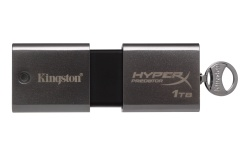
\includegraphics[width=0.25\linewidth]{eps/USB.eps}
%\end{figure}
}


%\footnote{Because of data reshiffling now H1 data temporary is only on tape}	


\frame{\frametitle{OPAL data in MPP: Bits statistics}
%\hspace{6cm}
\begin{columns}[c]
\column{0.85\linewidth}
Data are  ROOT/PAW ntuples, ASCII files, etc. Particle level NLO Monte Carlo is available for multiple generators.
\begin{table}\centering\bf\begin{tabular}{|c|c|c|}\hline
{\color{maroon}           } & {\color{maroon}   MPCDF     }          \\\hline\hline
{\color{maroon}Files:      }&{\color{maroon}   112k  } \\
{\color{maroon}Volume:     }&{\color{maroon}   $92 TB$ ($91.9\times10^{12}$ bytes)} \\
{\color{maroon}Work area:  }&{\color{maroon}    yes       } \\
{\color{maroon}Access:     }&{\color{maroon}   Worldwide  } \\
{\color{maroon}Protocols: } &{\color{maroon}   Multiple, see list   } \\
{\color{maroon}Auth:      } &{\color{maroon}   Grid certificate with  } \\
{\color{maroon}      } &{\color{maroon}    OPAL VO membership } \\\hline
\end{tabular}
\end{table}
\column{0.15\linewidth}
\rotatebox{90}{
\includegraphics[height=0.40\linewidth,width=2.8\linewidth]{eps/MPCDF}}
\end{columns}


Available at:
\begin{itemize}
\item gsidcap://grid-srm.rzg.mpg.de:22128/pnfs/rzg.mpg.de/data/opal
\item grid-gftp2.rzg.mpg.de 
\item davs://grid-dav.rzg.mpg.de:2880//opal
\item \dots
\end{itemize}

}





\frame{\frametitle{MPP model for software preservation}
%Explicit effort put to make software it work in the next 10-15 years.
%Previous efforts and high quality of code made it possible.%  porting  was possible.

Key ideas:
\begin{itemize}
\item Rely on industry, not HEP-only standards.
\item Enable integration and compatibility with new physics software, e.g. data bases and Monte Carlo generators.
%\item ISO image of full operating system relying on Intel $x86$  architecture to assure easy usage.
\item {\bf Make software analysis-ready}
\end{itemize}


}






%\frame{\frametitle{OPAL software in MPP}
%\begin{itemize}
%\item Full chain for reconstruction of raw data to PAW/ROOT ntuples was resurrected.
%\item Main software for the analysis of early preserved and reconstructed data is vanilla PAW or ROOT(via h2root).
%\item Additional software includes:
%\begin{itemize}
%\item event display;
%\item Monte-Carlo generation packages;
%\end{itemize}
%\end{itemize}
%}



\frame{\frametitle{OPAL software }
Not much to say about MPP specifically\dots But that is good!
\begin{itemize}
\item Huge and {\bf \color{red} successful } effort by Matthias Schr\"{o}der to keep the code compatible with modern systems.
\item High quality code.
\item Tests to put software in VM were done. 
\end{itemize}
}



\frame{\frametitle{OPAL software extension}
One can go ZEUS/JADE way:
\begin{itemize}
\item 	Add modern MC generators and conversation utility for modern format. Easy: OPAL uses ASCII based HEPEVT-like format.
\item   Add virtualisation. Things are working, but no image so far. Biggest problem is event display.
\end{itemize}
Not completed, but one can imagine how things should look like.
}

\section{Conclusions}

\frame{\frametitle{MPP Data Preservation summary}
\begin{itemize}
\item Huge work was done to preserve OPAL data and software.
\item The data in ntuples is accessible in  MPCDF and is {\bf\color{red}analysis-ready}.
\item Virtualisation is on the way in MPP (and CERN).
\item {So far MPP is involved mainly in the analysis
\begin{itemize}
\item Jet physics.
\item Collective phenomena.
\end{itemize}
}
\end{itemize}

}
\section{Data Preservation applications}
\frame{\frametitle{OPAL Data Preservation applications}
\begin{itemize}
\item Hadronisation/non-perturbative effects.
\item Fundamental questions of QCD.
\item Exotic hadronic states.
\item Flavour physics.
\item \dots
\end{itemize}
}

\section{What other experiments can learn from OPAL DP}


\frame{\frametitle{Software}
\begin{itemize}
\item Quality of code is important.
\item Compatibility with modern experiments!
\item Involvement of experts (M.~Schr\"{o}der)
\item Promotion: an anecdotal case of spending two conference evenings advertising preserved LEP data and its availability for re-analysis.
\end{itemize}
}



%\frame{\frametitle{This part should be considered as an opinion}



%%}

\frame{\frametitle{ \   }
\begin{center}{\Huge Some opinions}\end{center}
}


\frame{\frametitle{Some thoughts on DP in general}
Software:
\begin{itemize}
\item Software still requires some efforts. Can we join efforts?
Something like software repository with a proper package management system would 
be a nice idea. %Why don't we have the HEP software in proper formats? All these installation scripts and 
%"export hundred variables" before it works is just annoying. 
The technologies to do that (i.e. rpm/yum/etc) 
already 20+ years on the market, but still not in HEP.
\end{itemize}

}

\frame{\frametitle{Some thoughts on DP in general}
DP plans:
\begin{itemize}
\item Abstraction is good, but there is a huge difference between number of abstract concepts and 
actual examples of implementation. 
%In HEP we know that some detectors are better that others from the experience,
%but it is not the case for DP. For the detectors we have resolution/coverage/reading time/etc. Mostly about physics.
%Should one expect physics in the plans?
\end{itemize}

}


\frame{\frametitle{Some thoughts on DP in general}
%OK, OPAL DP is quite advanced. But, in the same time, the collaboration has ended in 2007.
%10 years is enough to understand the chalanges of analysis of data after 10 years..
Some technical and sociological problems:
\begin{itemize}
\item Missing or obscure  technical documentation. %While OPAL primer does exist, it doesn't cover everything.
%Thought one can admit the documentation from OPAL is quite good.
\item Some very specific details of  physics of old experiments can be  forgotten.
%e.g.\ absence of jet $p_{T}$ cut in $e^{+}e^{-}$ confuses people working with hadronic colliders.
\item The terminology in 1980, 2000 and now is different, old methods are renamed, etc.    This slows down communication and understanding of documentation.
%e.g.\ Monte Carlo tuning method by DELPHI (Z. Phys., C73 (1996) 11-60) has 293 citations overall, 2 in 2016.
%The tool based on the method
%   Professor (Eur.Phys.J. C65 (2010) 331-357) has 217 citations overall 22 in 2016.
%Ironically data sets from DELPHI are intensively used with the framework.
\end{itemize}
}

\frame{\frametitle{Some thoughts on DP in general}
More sociological problems:
\begin{itemize}
\item Manpower in not actually that severe problem per se. But the concentration is.
 With low spatial concentration of knowledge, there are few people that can be asked about specific things, discussions via mail exchange are not that productive.
The learning curve becomes too long. Should bigger laboratories like CERN and DESY be more involved? Some events for young physicists? Open data for older experiments?        
\item Long duration of any potential analysis because of involvement of members in other projects. The duration of any analysis more than 12 months 
implies that it cannot be advertised as a master or bachelor thesis. This rejects a very important source of manpower or requires more intensive supervision that for the 
running experiments. Could multiple supervisors and multiple master students  per  project be a solution? Thought the publication of the result should be mandatory.

%\item In the end DP has some sociological problems as well.
\end{itemize}

}




\frame{\frametitle{Some thoughts on DP in general}
More sociological problems:
\begin{itemize}
\item Doesn't matter how good are new technologies, it is still hard to convince experienced people to use them.
There is a fear the efforts to learn these things will be wasted. 
Good examples are Grid tools or PROOF.
\end{itemize}
}


\frame{\frametitle{Some thoughts on DP in general}
\begin{itemize}
\item Often the investments of manpower in earliest and not very precise measurements are 
much bigger than investments in the DP or even in the later results.
Emphasise of DP importance could fix this imbalance and make later/after-end-of-datataking precise analyses easier.
Analysis preservation addresses the issue.
\item A bit of sociological problem.

%\item In the end DP has some sociological problems as well.
\end{itemize}

}


\end{document}

